\begin{figure*}[h]
	\begin{subfigure}{0.48\textwidth}
		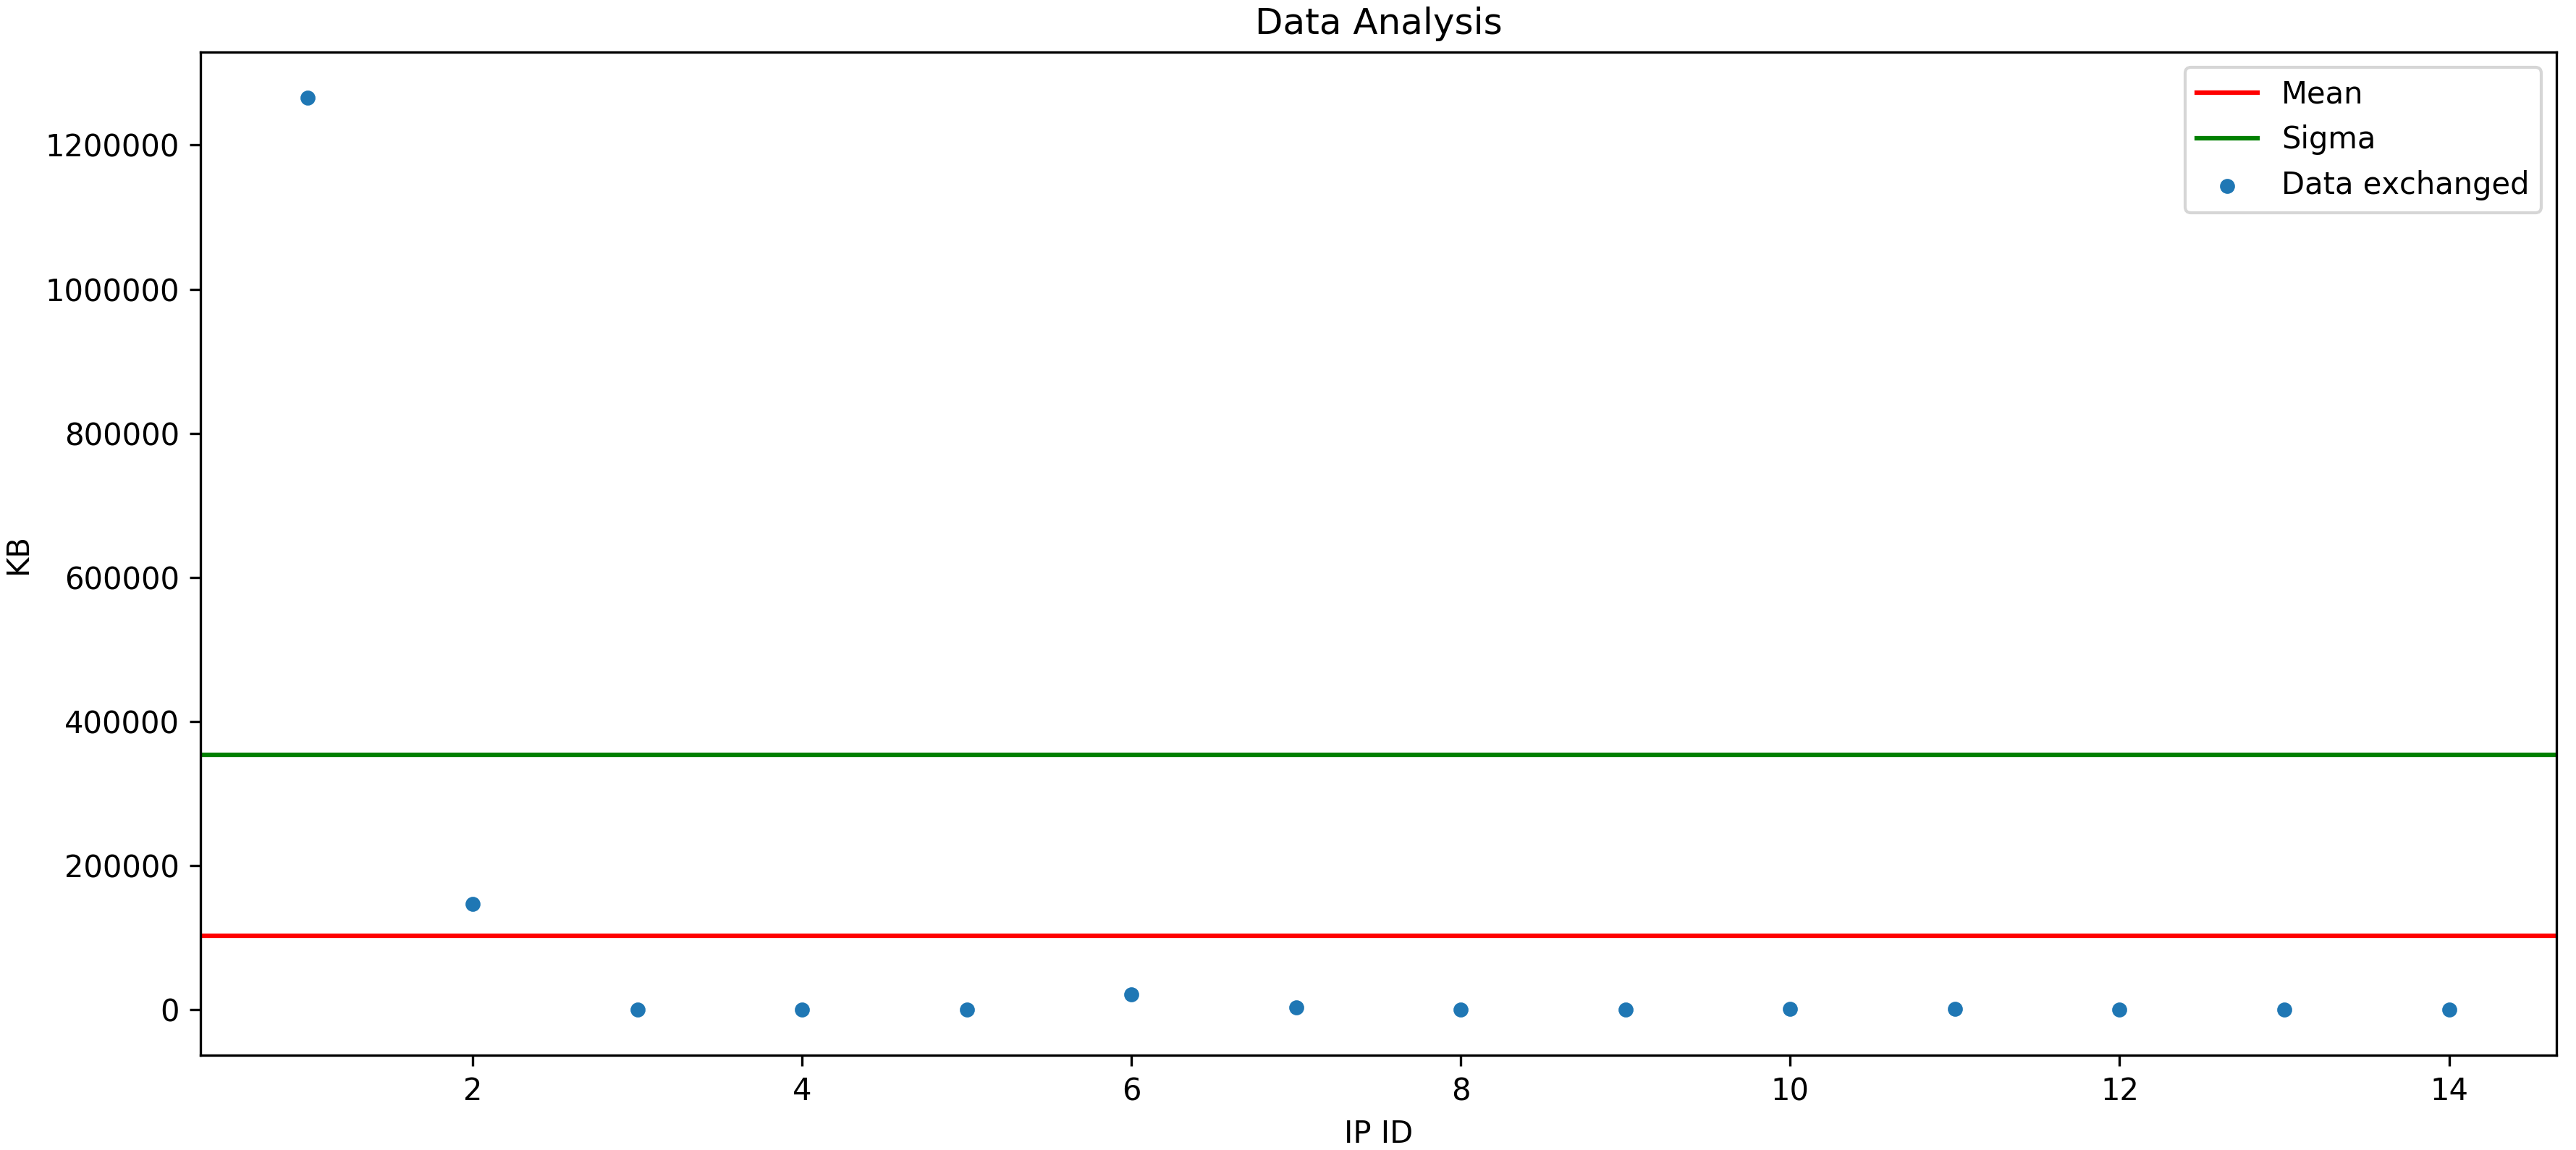
\includegraphics[width=\textwidth]{imgs/DDoSMixed-data_analysis}
		\caption{DDoS Data Analysis} 
		\label{fig:ddos_data}
	\end{subfigure}
	\hspace*{\fill} % separation between the subfigures
	\begin{subfigure}{0.48\textwidth}
		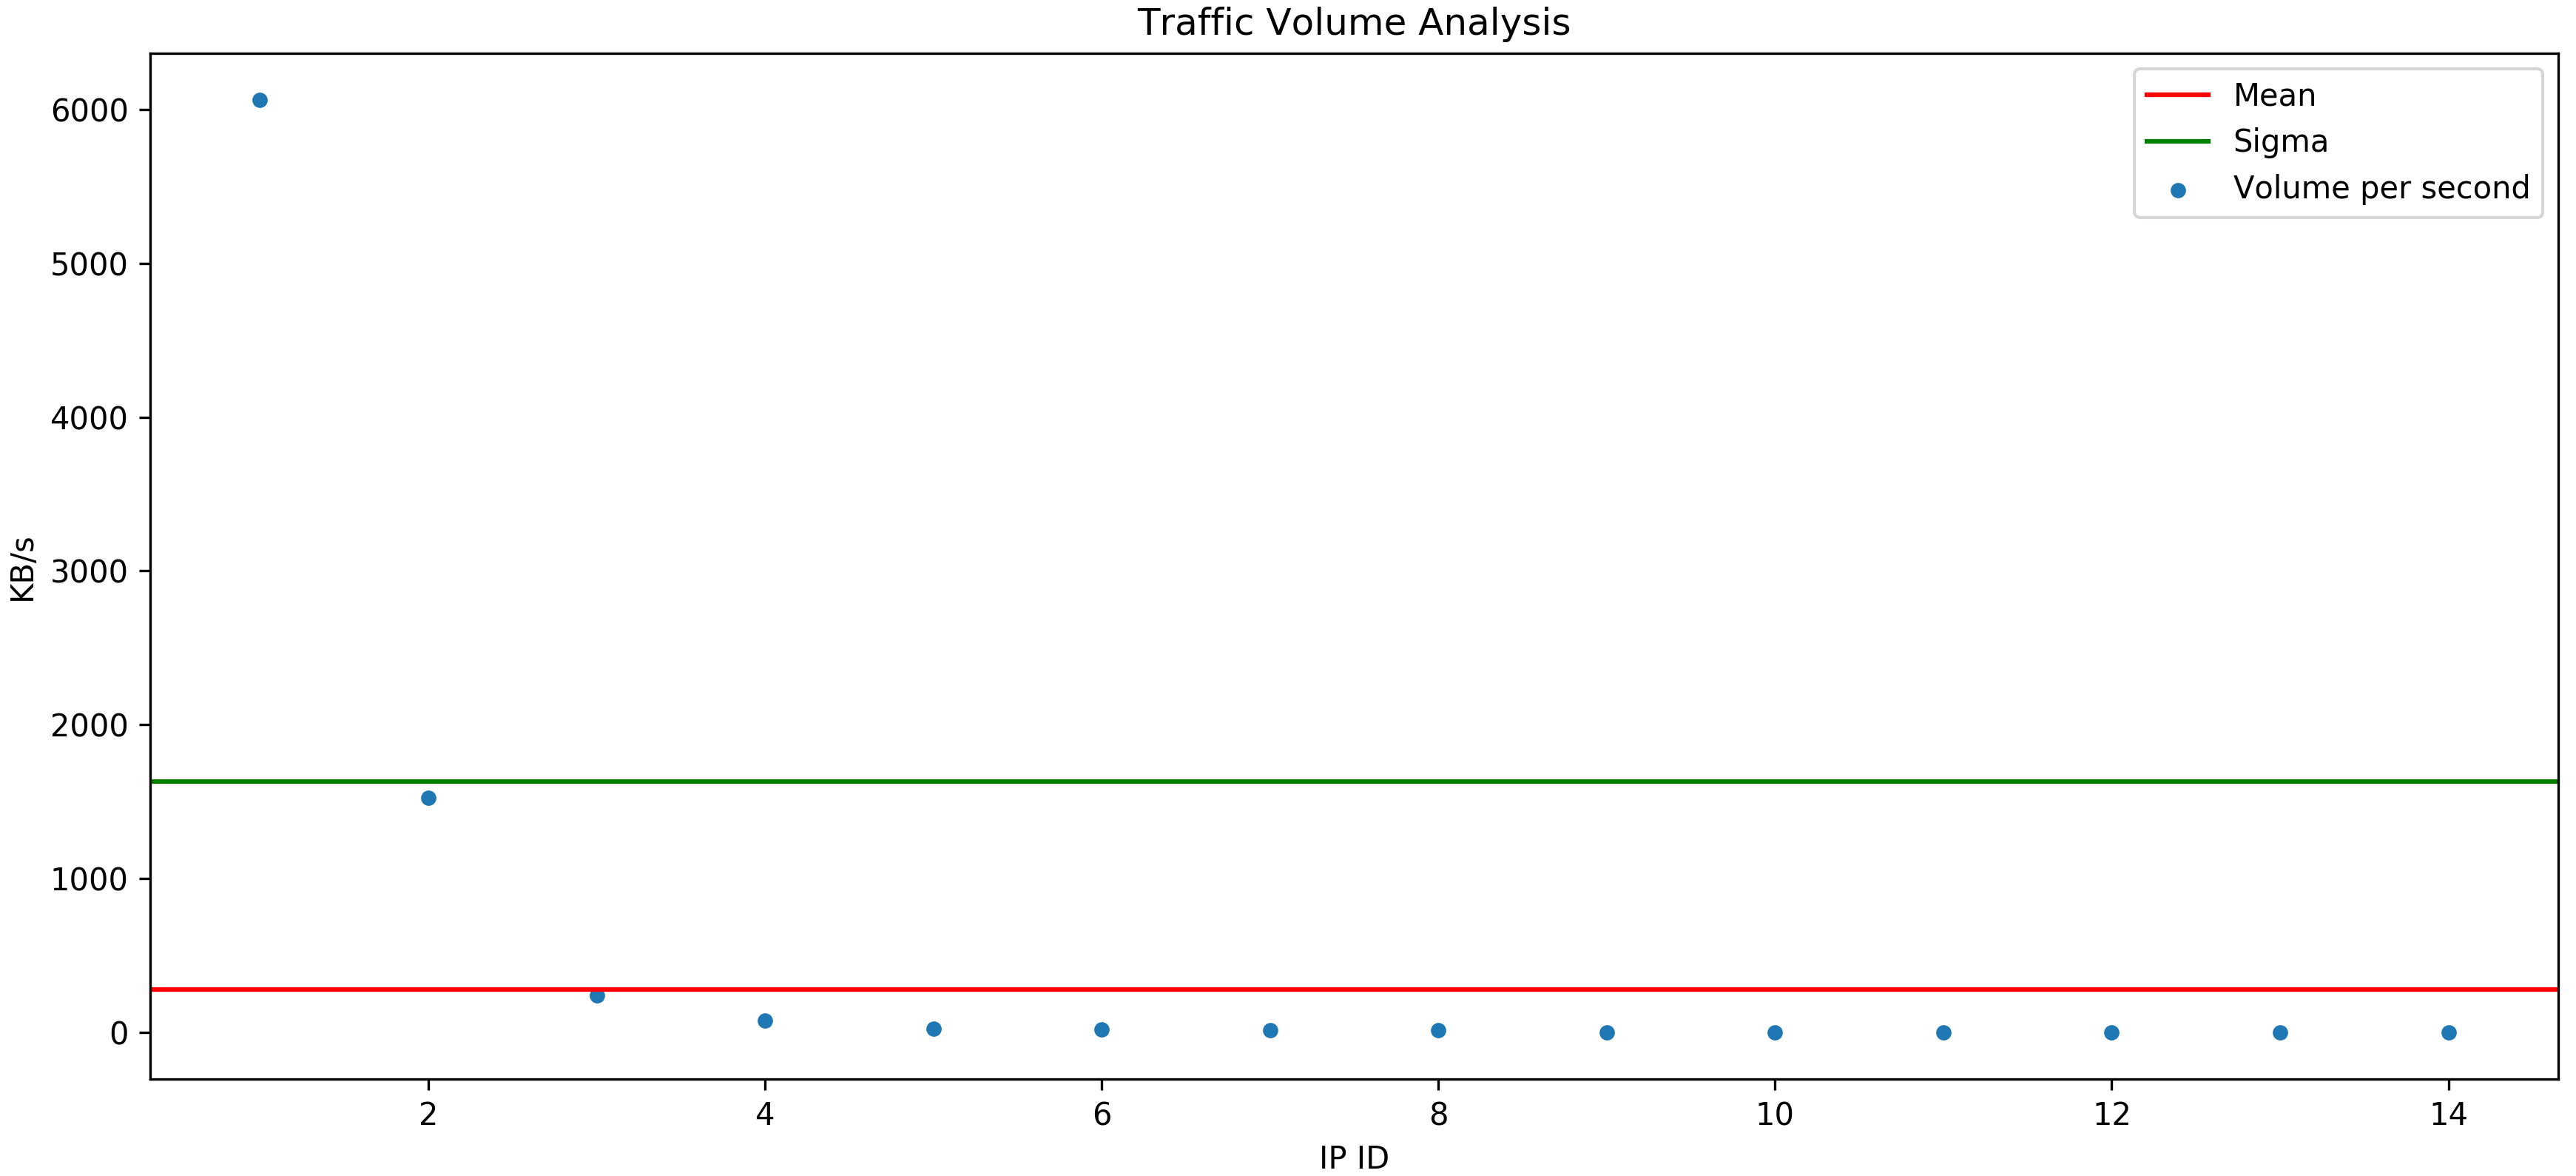
\includegraphics[width=\textwidth]{imgs/DDoSMixed-volume_analysis}
		\caption{DDoS Volume Analysis} 
		\label{fig:ddos_volume}
	\end{subfigure}
	\caption{DDoS attack Analysis}
	\label{fig:ddos_analysis}
\end{figure*}

\section{Performance Analysis}
\label{sec:perfanalysis}
In our tool we have developer a \textit{script} which records timestamps and duration time of big data analysis in a \texttt{.csv} file, called \texttt{PerformanceHistory.csv}. The \textit{script} mentioned before is used in order to figure out the time of analysis. 
The environment in which we tested our tool is a cluster of the University of Verona, running Ubuntu 18.04.1 LTS, it has an Intel Xeon Processor Skylake (4 cores @ 2,6 GHz) and a RAM memory of 7880 MiB for a single node, in its total configuration it has ten VCore and 60GB of RAM memory. 
We have never observed a total usage of more of 10\% CPU using \texttt{top} command and, in general, memory usage is often below 3000 MiB.
%% TODO performance scritte bene guardando pagina del cluster 
Using our script called \texttt{PerformanceAnalysis.py} we managed to plot the time elapsed to generate and analyze the datasets listed into Tab. \ref{tab:dataset_info}: results are reported into Fig. \ref{fig:datasets_statistics}.
We can immediately see that the generation time is much greater for attack datasets: this is justifiable because of the greater size, considering multi-user disk accesses.
Talking about analysis statistics, we can see a spike in \textit{ddos\_atk} and \textit{no\_atk} datasets. Here, long cluster timeouts during Pig Latin script execution play a great role, and we cannot have much control over it. Without that problem, analysis of the datasets would have taken much less time.

\begin{figure}[ht]
	\centering
	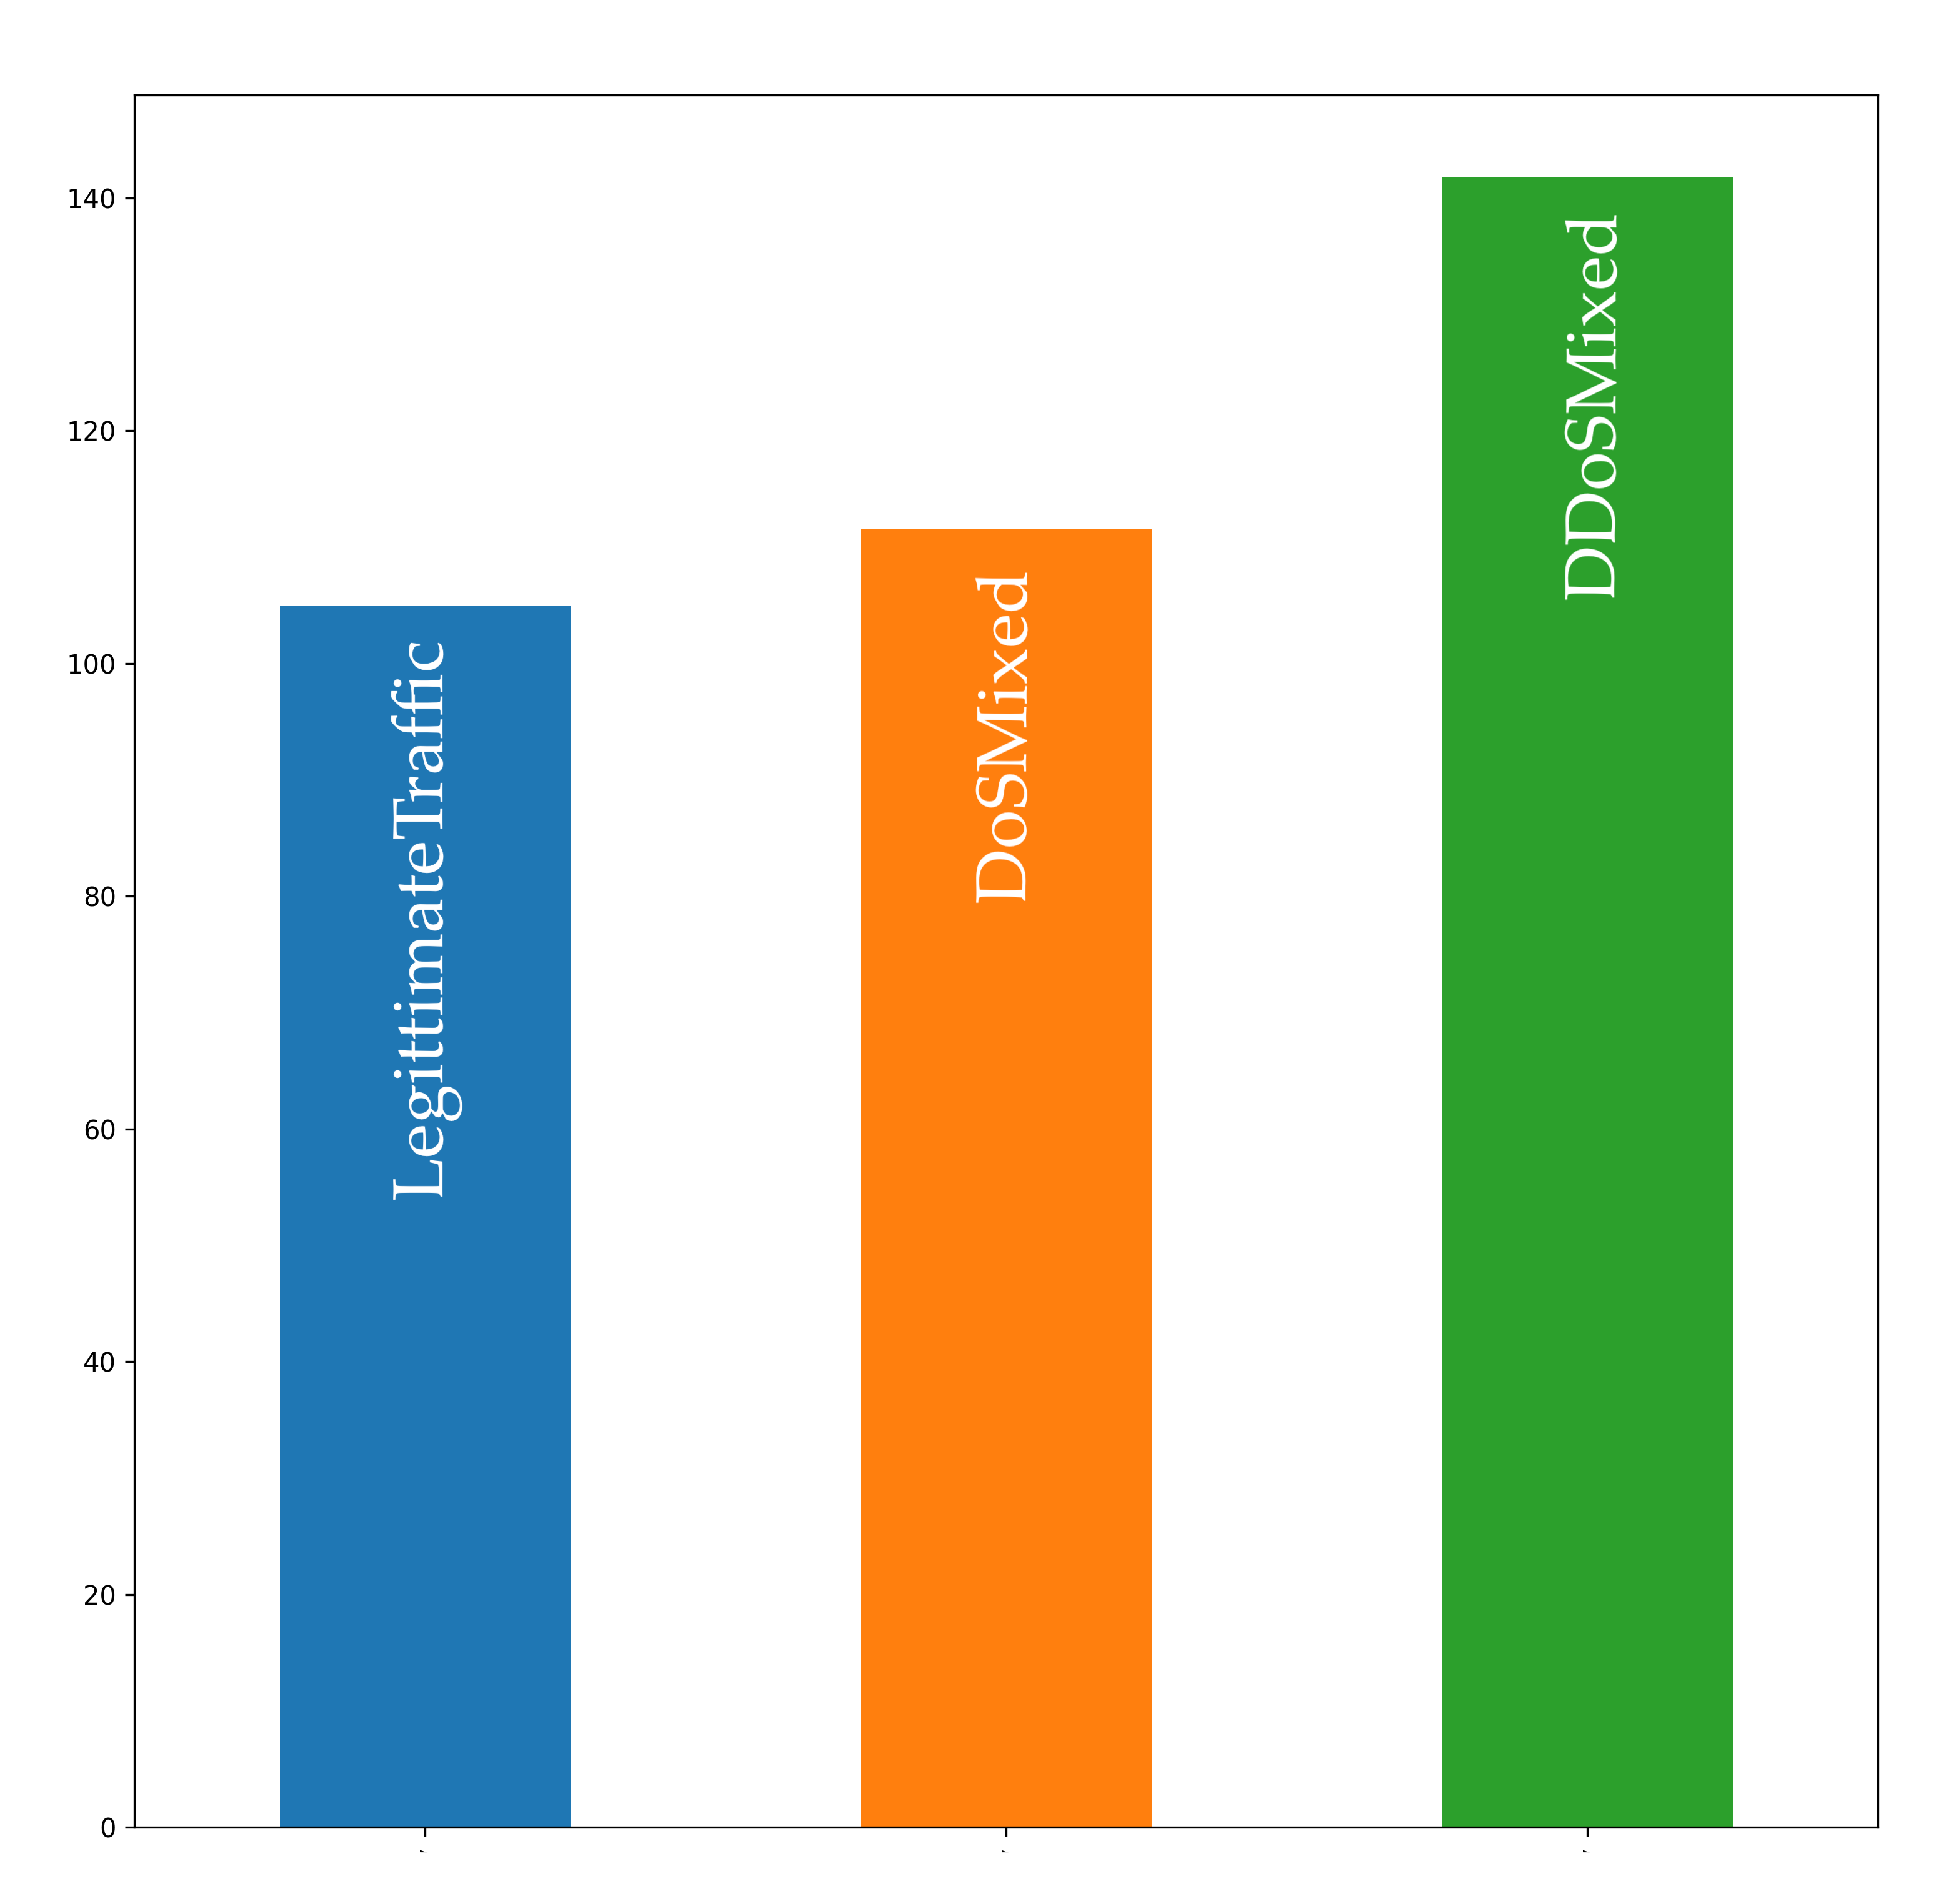
\includegraphics[scale=0.49]{imgs/analysis_stat.png}
	\caption{Performance Analysis} 
	\label{fig:analysis_stats}
\end{figure}

\begin{table}[!htbp]
\centering
\begin{tabular}{|l|l|c|}
\hline
\textbf{Dataset} & \textbf{Description}                              & \textbf{Size} \\ \hline
LegitimateTraffic         & Traffic log in normal conditions. & 316 KB        \\ 
DoSMixed        & Traffic log during a DoS attack.                   & 89 MB       \\ 
DDoSMixed        & Traffic log during a DDoS attack. & 612 MB        \\ \hline
\end{tabular}
\caption{Datasets Info}
\label{tab:dataset_info}
\end{table}
